\section{Hopfield Network}
1982 yılında John Hopfield tarafından önerilmiştir. Hopfield ağı, birbirine bağlı nöronlardan oluşur ve her bir nöron diğer nöronlar ile bağlantılıdır. Enerji fonksiyonu adında bir fonskiyonu minimize etmeye çalışır. Bu fonksiyon, ağdaki her bir nöronun aktivasyon seviyesine ve nöronların arasındaki bağlantıların ağırlıklarına bağlıdır. Ağ, enerji fonksiyonunu minimize edecek şekilde nöronların ağırlıklarını değiştirir. Sürekli ve Kesikli olmak üzere iki türü vardır.

\begin{figure}[h]
    \centering
    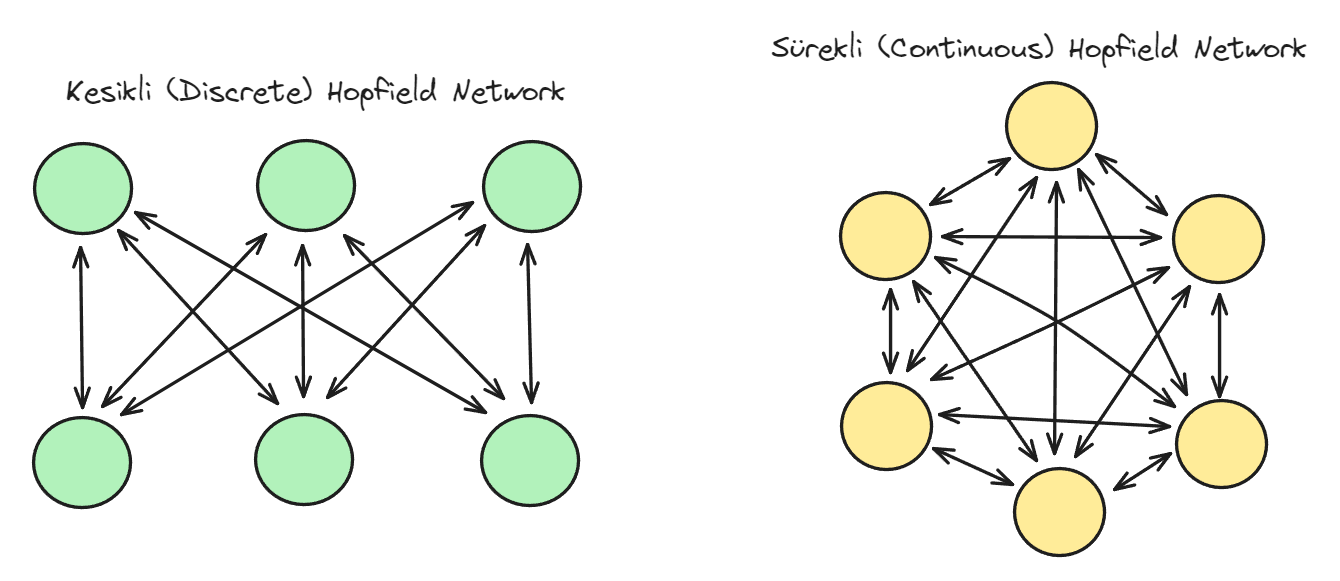
\includegraphics[width=1\textwidth]{images/hopfield_networks.png}
    \caption{Hopfield ağı mimarisi.}
    \label{fig:enter-label}
\end{figure}

\begin{itemize}
    \item \textbf{Kesikli Hopfield Ağları:} İkili giriş çıkış değerlerini kullanır. Nöron çıkışları bir eşik değere göre belirlenir. 
    \item \textbf{Sürekli Hopfield Ağları:} Sürekli gerçek değerleri kullanır. Nöronların çıkışları bir aktivasyon fonksiyonu ile belirlenir.
\end{itemize}

\subsection{Çalışma Adımları}
\begin{enumerate}
    \item Başlangıçta ağın bellek durumunu temsil eden rastgele belirlenmiş bir dizi giriş örneği ile başlar.
    \item Her adımda ağdaki nöronlar güncellenir. Her nöron, bağlı olduğu diğer nöronların değerlerine göre kendi çıkışını günceller.
    \item Ağın enerji fonksiyonu, ağdaki nöronların ve aralarındaki bağlantıların durumuna dayanır. Ağın enerji seviyesi, her bir örnek için bir enerji değeri üretir. Ağ, enerji fonksiyonunu minimize etmeye çalışır.
    \item Ağ, enerjisini azaltan veya sabit tutan bir duruma ulaşıncaya kadar güncellenmeye devam eder. Bu durum, ağın örnekleri hatırlayabileceği bir halde olduğunu gösterir.
\end{enumerate}

\newpage